\chapter*{ \centering Task 5}
\addcontentsline{toc}{chapter}{Task 5}

\section*{Practical Implementation}

\textbf{Threats that were found after performing scan}\\
	\begin{figure}[H]
	\centering
	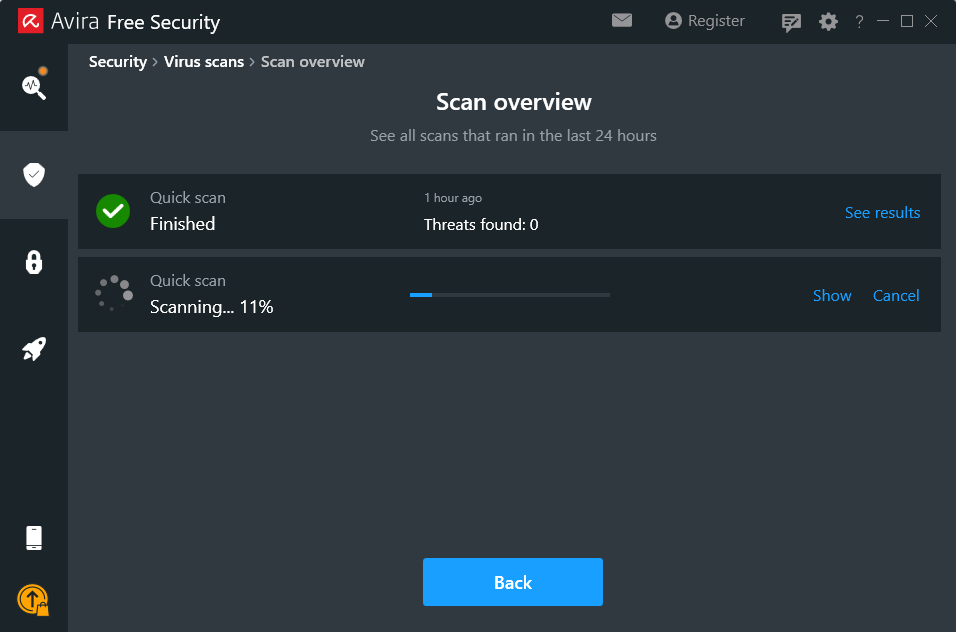
\includegraphics[scale=0.5,height=5cm]{"/home/kali/Documents/latex_files/cyber_rp/graphics/scanner.png"} \\
	\caption{Scanning for Threats}
\end{figure}
\begin{enumerate}
	\item
	 Threat Type: Trojan\\
	Location: \path{C:\ ProgramData \ AvastSvcXoF \ AvastAuth.dat }\\
	Severity: High \\
	Action Taken: Quarantined and deleted by antivirus software. \\
	\item
	Threat:Available space to free up\\
	Severity:Medium\\
	Action:Cleared unused space

\end{enumerate}

\newpage
\textbf{IMPORTANCE OF KEEPING ANTIVIRUS AND SPYWARE SOFTWARE UPDATED}\\
The number viruses and spyware are on the rise everyday therefore it is our duty to keep up with it. Our software therefore has to be up to date so as to keep up with the fast pace growth of the viruses. This will help keep our machines safe from the harm viruses and spyware.\\

\textbf{SCHEDULE FOR REGULAR SCANS AND UPDATES}
\begin{enumerate}
	\item	Scans and updates should be done at least once a week
	\item	After an external device has been inserted and data or information has been fetched from it
	\item After a new software has been installed
\end{enumerate}

\textbf{EFECTIVENESS OF THE INSTALLED SOFTWARES}\\
The software requires a premium to be more effective. The free versions (which we used) wasn’t as effective as would be needed.